\chapter{Transfering safe policies}
\label{chapter:slsp}

In this chapter, we propose to \idx{transfer} a safe strategy to initiate the first \idx{dialogue}s. We introduce an extension of the classic $\egreedy$-greedy exploration strategy. We test the algorithm on a slot-filling application.
%!TU: un peu court

\section{Motivation}

During its early steps of learning, an \gls{RL} based \idx{dialogue} \idx{agent} does a lot of exploration that may lead to penalising behaviours. However, the first interactions between a \idx{user} and a \gls{DS} are crucial to gain trust. To improve \idx{jumpstart} performance of an \gls{RL} \idx{agent}, one can \idx{transfer} a strategy~\parencite{taylor2009transfer,LazaricSurvey}. In \idx{dialogue}, the strategy focuses on the success of the \idx{dialogue} while minimising its length~\parencite{Chandramohan2010,Casanueva2015,Genevay2016}. Rushing the \idx{dialogue} may be problematic with some \idx{user}s and induce premature \idx{dialogue} hangups\index{hangup}. First, it could lead to the loss of this \idx{user} once for all. Second, the lack of sucessful \idx{dialogue}s may affect the learning speed of the \gls{RL} \idx{agent}. To this extend, we introduce a novel algorithm: $\egreedy$-safe. It \idx{transfer}s a safe strategy which avoid any critical \idx{dialogue act} to prevent the aforementioned problems.


\section{\texorpdfstring{$\epsilon$}{E}-safe}

\begin{figure}
    \centering
    %\bigcentering
    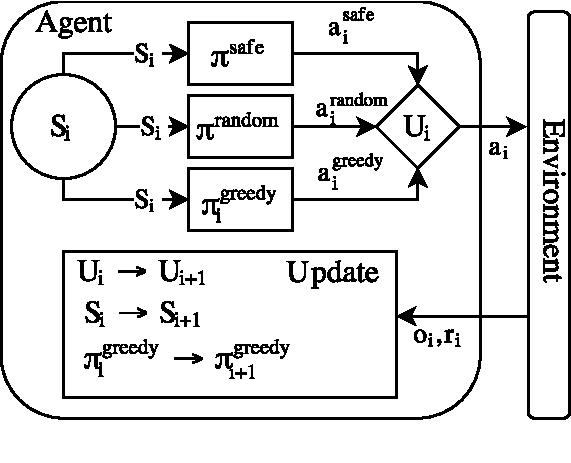
\includegraphics[width=0.6\columnwidth]{sources/contribution/slsp/transfer7}
    \caption{$\egreedy$-safe algorithm.} %combined with an online off-policy RL algorithm: online phase.}
    \label{fig:qlearning}
\end{figure}

$\egreedy$-safe (\Cref{fig:qlearning}) is a $\Q$-learning algorithm~\parencite{Watkins92q-learning} where each action is decided by a randomly chosen policy among the \idx{greedy} policy, an exploratory policy and the \idx{transfer}red \idx{safe policy}. The safe policy may be a \idx{handcrafted} or a trained policy.

\section{Experiment}

\begin{figure}
        \centering

    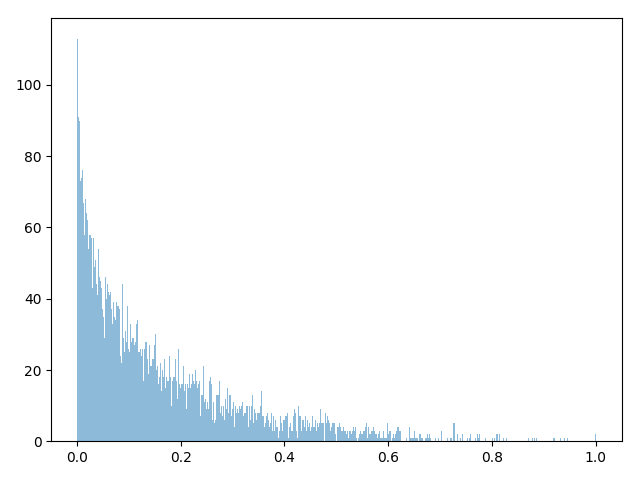
\includegraphics[scale=0.35]{sources/contribution/slsp/distribusers}
    \caption{Half-Gaussian distribution of $p$ values.}
    \label{distribusers}
\end{figure}


\begin{figure}
    \begin{center}

    \subfloat[Dialogue score]{
        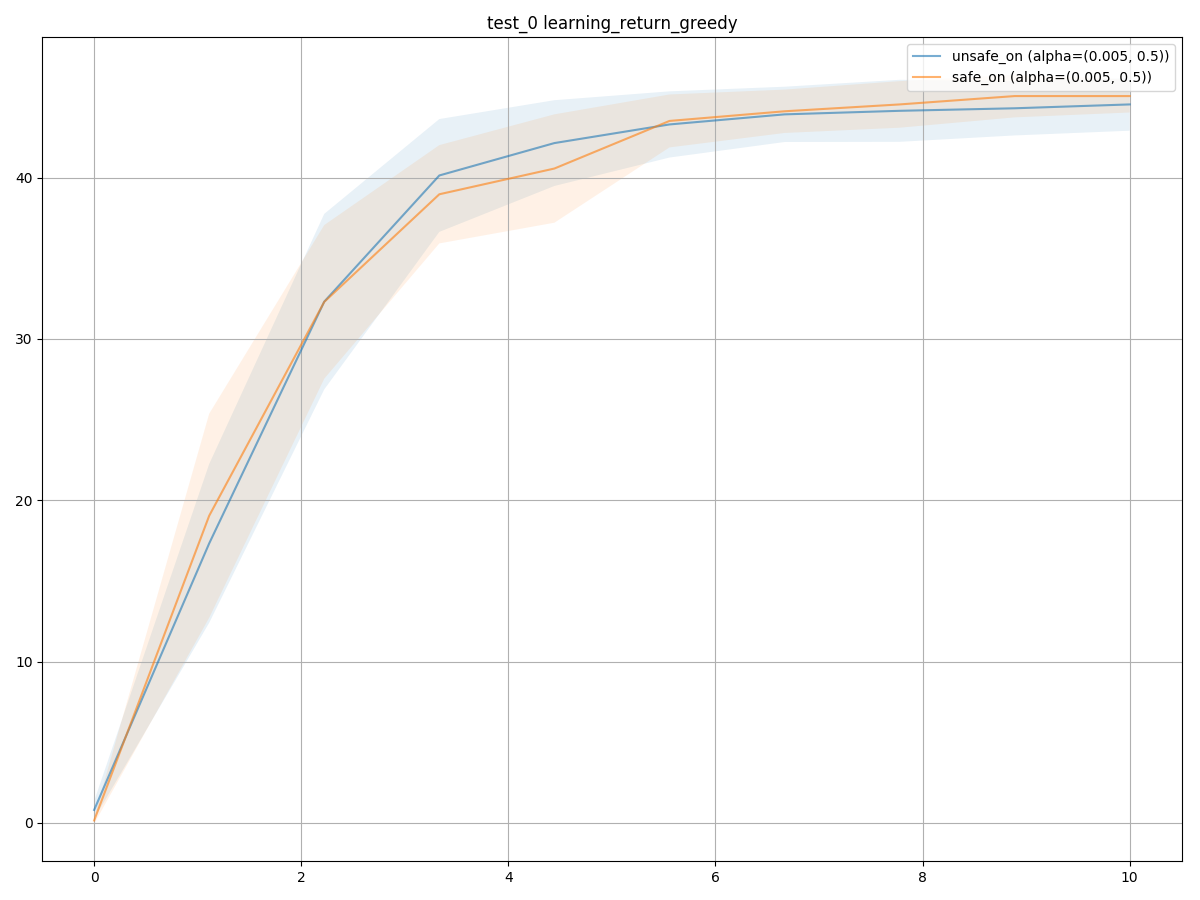
\includegraphics[scale=0.25]{sources/contribution/slsp/retgreed}
        \label{retgreed}
    }\\
    % spacing between the subfigures
    \subfloat[Success frequency]{

        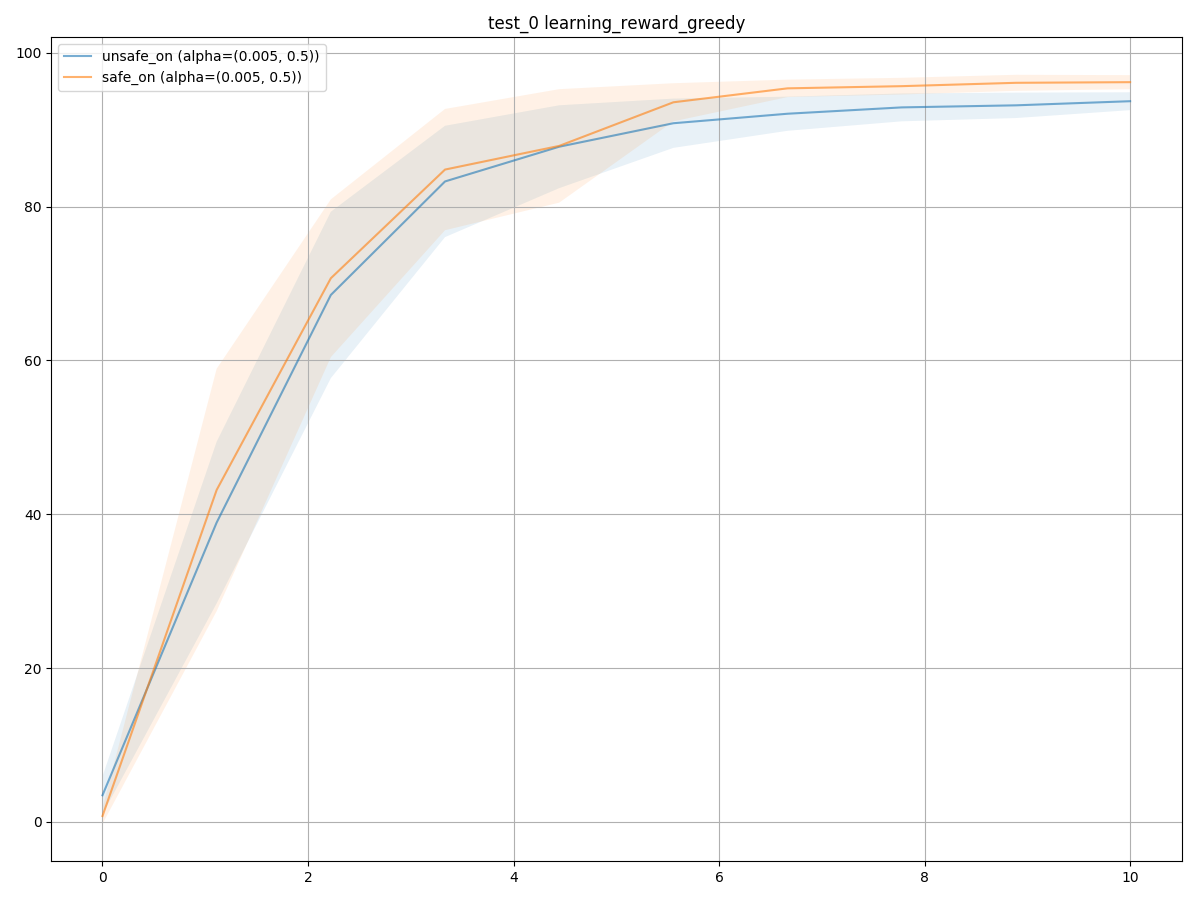
\includegraphics[scale=0.25]{sources/contribution/slsp/rewgreed}
        \label{rewgreed}
    }


    \caption{Performance of the \idx{greedy} policies.}
    \label{fig:exampleexecution}
\end{center}
\end{figure}

We test our algorithm on a \idx{slot-filling} application. It is a simpler version of the one use in \Cref{chapter:nips}. The \idx{agent} asks for slot values, but this time, slot by slot in a fixed order. Several acts are available:

\begin{itemize}
    \item \texttt{ask-next}: ask next slot (with \gls{ASR} errors).
    \item \texttt{repeat-oral}: repeat current slot (with \gls{ASR} errors).
    \item \texttt{repeat-numpad}: repeat current slot using numeric pad (without \gls{ASR} errors).
    \item \texttt{summarize-inform}: summarise slots values and return the form result. If values are correct, the \idx{dialogue} ends successfully, if not, the slot values are reset and the \idx{dialogue} continues from the first slot.
\end{itemize}

\texttt{repeat-numpad} is an unsafe action: the \idx{user} hangups\index{hangup} with probability $p$. For each new \idx{user}, $p$ is randomly generated. An histogram of $p$ values is displayed \Cref{distribusers}.

We define two \idx{handcrafted} \glspl{DS}. The \texttt{safe} system uses \texttt{repeat-oral} if the recognition score is bellow 0.5, otherwise \texttt{ask-next}, or \texttt{summarize-inform} after the last slot; The \texttt{unsafe} system uses \texttt{repeat-numpad} instead. We compare two $\egreedy$-safe \idx{agent}s. \texttt{safe-on} uses \texttt{safe} as \idx{transfer}red policy while \texttt{unsafe-on} \idx{transfer}s the \texttt{unsafe} policy.


We test \texttt{safe-on} and \texttt{unsafe-on} with 10 randomly generated \idx{user}s, for 1000 \idx{dialogue}s. We repeat the experiment 10 times. We display the performance of the \idx{greedy} policies. The \idx{dialogue} score (reward penalised by \idx{dialogue} length) is plotted on \Cref{retgreed} while the \idx{dialogue} success (reward only) is plotted on \Cref{rewgreed}. We see that despite a slightly difference on the \idx{dialogue} success, the \idx{dialogue} score is the same. That means $\egreedy$-safe does not improve the learning speed of the \idx{greedy} policy even if it is conservative enough to keep the \idx{user} in the \idx{dialogue} by avoiding catastrophic acts.
%

